\subsection{Translation and Ribosomal Synthesis}
Lastly, we turn our attention to the process of synthesizing new proteins,
translation. This process stands as a good candidate for potentially limiting
growth since the synthesis of new proteins relies on the generation of
ribosomes, themselves proteinaceous molecules. As we will see in the coming
sections of this work, this poses a "chicken-or-the-egg" problem where the
synthesis of ribosomes requires ribosomes in the first place.

We will begin our exploration of protein translation in the same spirit as we
have in previous sections -- we will draw order-of-magnitude estimates based
on our intuition and available literature, and then compare these estimates
to the observed data. In doing so, we will estimate both the absolute number
of ribosomes necessary for replication of the proteome as well as the
synthesis of amino-acyl tRNAs. From there we consider the limitations on
ribosomal synthesis in light of our estimates on both the synthesis of
ribosomal proteins and our earlier results on rRNA synthesis.

\subsubsection{Protein Synthesis}
With the number of tRNA synthetases accounted for, we now consider the abundance
of the protein synthesis machines themselves, ribosomes. Ribosomes are enormous
protein/rRNA complexes that facilitate the peptide bond formation between amino
acids in the correct sequence as defined by the coding mRNA. Before we examine
the synthesis of the ribosome proteins and the limits that may place on the
observed bacterial growth rates, let's consider replication of the cellular
proteome.

While the rate at which ribosomes translates is well known to have a growth
rate dependence \cite{dai2018} and is a topic which we discuss in detail in
the coming sections. However, for the purposes of our order-of-magnitude
estimate, we can make the approximation that translation occurs at a rate of
$\approx$ 15 amino acids per second per ribosome (BNID: 100233). Under this
approximation and assuming a division time of 5000 s, we can arrive at an
estimate of $\approx 10^4$ ribosomes are needed to replicate the cellular
proteome, shown in \FIG{protein_synthesis}(B). This point estimate, while
glossing over important details such as chromosome copy number and
growth-rate dependent translation rates, proves to be notably accurate when
compared to the experimental observations (\FIG{protein_synthesis}(B)).

\begin{figure}
    \begin{fullwidth}
    \centering{
        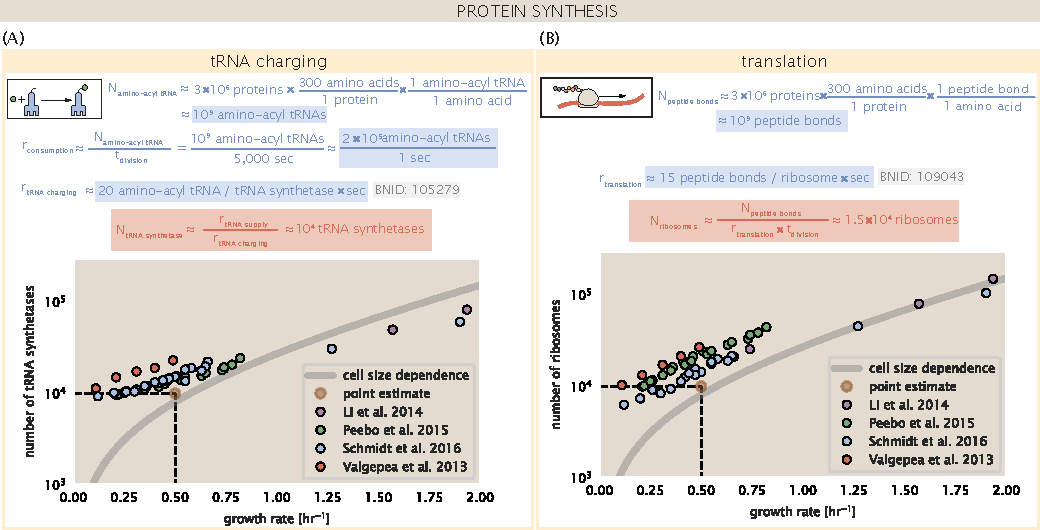
\includegraphics{main_figs/fig8_protein_synthesis.pdf}
        \caption{\textbf{Estimation of the required tRNA synthetases and
        ribosomes.} (A) Estimation for the
        number of tRNA synthetases that will supply the required amino acid
        demand. The sum of all tRNA synthetases copy numbers are plotted as a
        function of growth rate ([ArgS], [CysS], [GlnS], [GltX], [IleS], [LeuS],
        [ValS], [AlaS]$_2$, [AsnS]$_2$, [AspS]$_2$, [TyrS]$_2$, [TrpS]$_2$,
        [ThrS]$_2$, [SerS]$_2$, [ProS]$_2$, [PheS]$_2$[PheT]$_2$, [MetG]$_2$,
        [lysS]$_2$, [HisS]$_2$, [GlyS]$_2$[GlyQ]$_2$). (B) Estimation of the
        number of ribosomes required to synthesize 10$^9$ peptide bonds with an
        elongation rate of 15 peptide bonds per second. The
        average abundance of ribosomes is plotted as a function of growth rate.
        Our estimated values are shown for a growth rate of 0.5 hr$^{-1}$.
        Grey lines correspond to the estimated complex abundance calculated at
        different growth rates. See Appendix \nameref{sec:SI_continuum_est} for a more
        detail description of this calculation.}
    \label{fig:protein_synthesis}
    }
    \end{fullwidth}
\end{figure}
